\documentclass{article}

% if you need to pass options to natbib, use, e.g.:
% \PassOptionsToPackage{numbers, compress}{natbib}
% before loading nips_2016
%
% to avoid loading the natbib package, add option nonatbib:
% \usepackage[nonatbib]{nips_2016}

% \usepackage{nips_2016}

% to compile a camera-ready version, add the [final] option, e.g.:
\usepackage[final]{nips_2016}

\usepackage[utf8]{inputenc} % allow utf-8 input
\usepackage[T1]{fontenc}    % use 8-bit T1 fonts
\usepackage{hyperref}       % hyperlinks
\usepackage{url}            % simple URL typesetting
\usepackage{booktabs}       % professional-quality tables
\usepackage{amsfonts}       % blackboard math symbols
\usepackage{nicefrac}       % compact symbols for 1/2, etc.
\usepackage{microtype}      % microtypography
\usepackage{amsmath}
\usepackage{graphicx}
\graphicspath{ {images/} }
\usepackage{subfig}
\usepackage{multirow}
\usepackage{algorithm}
\usepackage[utf8]{inputenc} % allow utf-8 input
\usepackage[T1]{fontenc}    % use 8-bit T1 fonts
\usepackage{hyperref}       % hyperlinks
\usepackage{url}            % simple URL typesetting
\usepackage{booktabs}       % professional-quality tables
\usepackage{amsfonts}       % blackboard math symbols
\usepackage{nicefrac}       % compact symbols for 1/2, etc.
\usepackage{microtype}      % microtypography
\usepackage{amsmath}
\usepackage{graphicx}
\usepackage{media9} 
\usepackage{caption}
% \usepackage{subcaption}
\usepackage{amsmath}
\usepackage{algorithm, algpseudocode}

\title{Zero shot learning of vector images}

\author{
  Nitish Kulkarni \\
  \texttt{nitishkk@cs.cmu.edu} \\
  \And
  Aditya Siddhant \\
  \texttt{asiddhan@cs.cmu.edu} \\
  \And
  George Tan \\
  \texttt{georget1@cs.cmu.edu} \\
}

\begin{document}
% \nipsfinalcopy is no longer used

\maketitle

\begin{abstract}
Use of neural networks for generation of images has gained popularity in recent times.  Most of the work in this area has targeted the modelling of pixel images. However, humans do not learn to draw images as matrix of pixels. They learn to represent abstract concepts present in an object using a sequence of strokes. We would therefore be trying to address the challenge of generating images or rather sketches in a vectorized manner given a pixel image of the object. Our goal would be train a generative model that learns to draw and generalize abstract concepts in a manner indistinguishable from humans. This is referred as 'Zero Shot' because the problem entails generation different sketch representations of previously unseen objects in pixel images during test time.
\end{abstract}


\section{Introduction}
Handwriting synthesis and hand-drawn sketch generation has been recently successful with deep neural networks. These deep neural networks include recurrent neural networks (RNN) with Long Short-term Memory (LSTM) \cite{LSTM}, Generative Adversarial Networks (GAN) \cite{GAN}, and Variational Autoencoders (VAE) \cite{journals/corr/KingmaW13} which all has demonstrated to generate human-level handwriting and sketches. Though, these methods are not suitable for generating sketches in a vectorized manner given a pixel image. When given an image, humans do not know the sequential, vector
representation of the image yet. Also, humans do not view sketches as just pixels image, but rather as sequence of strokes. From end-to-end, the goal is to train the machine to learn the high-level visual features of the pixel image and output a sketch images that is represented as sequence of vectors.

The goal stated above is naturally analogous to image captioning which is the problem generating natural sentences to describe a given image. Recent advances in image captioning lead to a generative model based on a deep recurrent neural network that combines advances in computer vision and machine translation. The model is the Neural Image Caption (NIC) \cite{DBLP:journals/corr/VinyalsTBE14} which is an end-to-end neural network with a Convolutional Neural Network (CNN) for feature learning on the image followed by a language generating RNN that uses the features from the CNN. In our problem of hand-drawn sketch generation given a pixel image, the sketch generation which are the sequence of vectors which is analogous to the language generation which are a sequence of words. We propose to borrow the ideas of the NIC model to create a deep neural network model to generate vectorized sketches given a pixel image.


\section{Related Work}
Generative models have shown recent success. RNNs with LSTM were used for handwriting synthesis i.e. generate handwritten characters for a given text \cite{DBLP:journals/corr/Graves13}. GANs, a framework to estimate generative models with an adversarial process, have been demonstrated to generate images of hand-written digits from MNIST \cite{MNIST}, faces from the Toronto Face Database \cite{TFD}, and various objects from CIFAR \cite{CIFAR}. VAEs, a generative model with an encoder and decoder architecture, can generate street view house numbers \cite{DBLP:journals/corr/GregorDGW15}.

Although free hand sketches have not received as much attention as pixel images, there has been quite a lot of work in recognition of free hand sketches using deep neural networks. Some works have tried to complete the sketch conditioned on first few strokes and try to build a system for guiding the free-form drawing of objects \cite{qdpaper} \cite{rcp2}. Other works have tried to retrieve the pixel image of an object given the sketch \cite{sketchydb} where one uses the deep features of the sketches \cite{rcp1}. One work has shown to mimic and recreate similar looking drawings from given drawings with generative models \cite{qdpaper}.

Recent improvements in image captioning include Show and Tell \cite{DBLP:journals/corr/VinyalsTBE14} and a Multimodal Recurrent Neural Network \cite{DBLP:journals/corr/KarpathyF14} that uses a architecture that is a CNN followed by a language generating RNN. To the best of our knowledge, there is no work that has used a multimodal deep learning approach to generate vectorized sketches using a pixel image.


\section{Method}
We would like to explore the extension of the multimodal NIC model \cite{DBLP:journals/corr/VinyalsTBE14} which is an end-to-end neural network with CNN for feature learning on the image followed by a language generating RNN that uses the features from the CNN. We use a CNN in order to learn visual features and to learn the latent variable that allows the LSTM RNN to generate the sketch image. In other words, the CNN learn the encoding of pixel image into the latent variable.

In order to to learn the sequence of strokes in a sketch to imitate human-like behavior, we use a RNNs and since Long Short-Term Memory (LSTM) \cite{LSTM} memory cells and Gated Recurrent Units (GRU) \cite{GRU} are well-suited to learn and predict on time series data, RNN can be used generate the strokes of an object's sketch. We plan to feed the encoding of pixel image into this RNN so that the stroke generation is conditioned on the pixel image.

\subsection{Data}
The input to the network is the pixel image represented as a matrix where $I$ is the pixel image and $I\in \mathbb{R}^{m\times n\times c}$ so the input image pixel has a height of $m$ and width of $n$ and $c$ number of channels depending whether the image is grayscale or RGB. The output of the network represents a sketch as a set of pen stroke actions as used by sketch-rnn \cite{qdpaper}. A single stroke action vector consists of five elements $(\Delta x, \Delta y, p_{1}, p_{2}, p_{3})$ where $\Delta x, \Delta y$ are the pen's offsets in the x and y direction to the next state, $p_{1}$ indicates that the pen is touching the paper, $p_{2}$ indicates that the pen is lifted from the paper, and $p_{3}$ indicates that the drawing is over. Given a sequence of the stroke action vectors, a sketch image can be constructed.

\subsection{Model}
\begin{figure}[h]
\centering
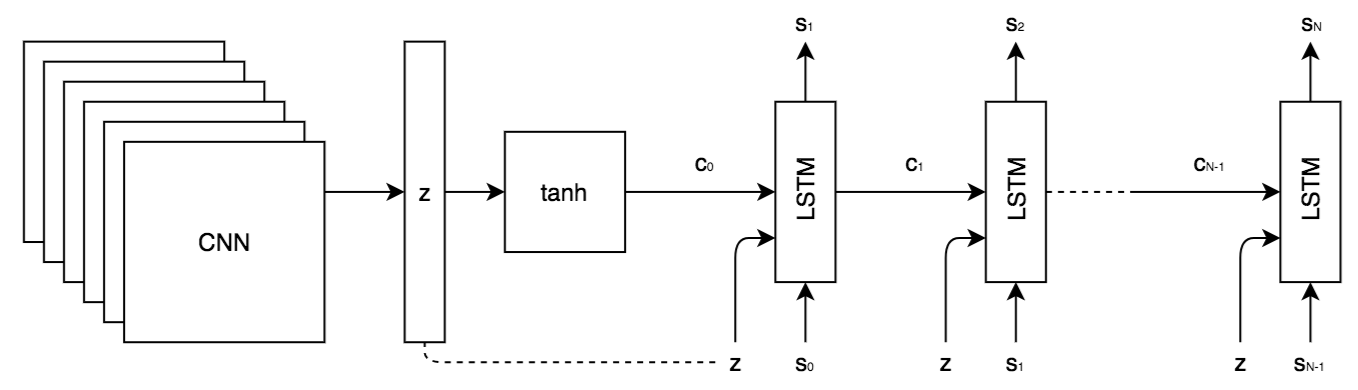
\includegraphics[scale=0.5]{images/model.png}
\caption{Diagram of the model}
\end{figure}

Let $I$ denote the input pixel image and $s = (s_{0}, ..., s_{N-1})$ be the vector sequence that constructs the sketch image where $s_{t} = (\Delta x_{t}, \Delta y_{t}, p_{t, 1}, p_{t, 2}, p_{t, 3})$. Then the forward procedure is
\begin{gather}
z = CNN(I), c_{0} = tanh(z), h_{0} = 0\\
[h_{t+1}; c_{t+1}] = LSTM([z;\hat{s_{t}}], [h_{t}; c_{t}])\\
y_{t+1} = Linear(h_{t+1}), y_{t+1}\in\mathbb{R}^{5}\\
\hat{s_{t+1}} = (y_{t+1,1}, y_{t+1,2}, softmax(y_{t+1,3}, y_{t+1,4}, y_{t+1,5}))
\end{gather}
for $t\in \{0, ..., N-1\}$ where z is the latent vector which is the output of the CNN "encoder" and the concatenated vector of z and $s_{t}$ is fed into the LSTM "decoder" to generate the next pen stroke action $s_{t+1}$ starting at $\hat{s_{0}} = (0,0,1,0,0)$. For the sketch image $s = (s_{0}, ..., s_{N-1})$ and predict output image $\hat{s} = (\hat{s_{0}}, ..., \hat{s_{N-1}})$, the loss is defined as
\begin{gather}
L_{total}(s, \hat{s}) = L_{R}(s, \hat{s}) + L_{CE}(s, \hat{s})\\
L_{R}(s, \hat{s}) = \sum_{t=0}^{N-1} (\Delta x_{t} - \Delta \hat{x_{t}})^{2} + (\Delta y_{t} - \Delta \hat{y_{t}})^{2}\\
L_{CE}(s, \hat{s}) = \sum_{t=0}^{N-1} \sum_{i=0}^{2} p_{t,i} log(\hat{p_{t,i}})
\end{gather}
where $L_{R}$ is the reconstruction loss i.e. the L2 loss of the offsets, $L_{CE}$ is the cross-entropy loss of the categorical output, and $L_{total}$ is the total loss which sums up the L2 loss of the offsets and the cross-entropy loss of the categorical output.

\subsection{Evaluation}
For quantitative evaluation, we first evaluate the final sketch drawn in terms of similarity to the human-drawn final sketches of the images by using couple of similarity metrics like cosine correlation and etc. This is testing if at least the drawn sketch corresponds to the correct image. Second, we evaluate if the stokes are human-like by the correlation between number of strokes model uses vs number of strokes humans use and for the corresponding strokes, compare the average time series similarity like dynamic time warping and time warp edit distance and cross correlation. For qualitative evaluation, we show some strokes and sketches of different input images and compared them with the ground-truth sketch.


\section{Experiments}
We would be using the Quick Draw dataset \cite{quickdraw} to train and evaluate our model. The dataset consists of over 50 million drawings of 200 objects contributed by over 15 million players who played Google’s drawing game, "Quick, Draw!". The dataset also captured the players' strokes and the sequence of the strokes to create each drawing. Right now, we are planning on using 100 categories with 10k sketches each for training and validation and 25 categories for testing. This might change depending on the computational complexity of our method and the resources that are available to us. In addition to this, we collected images from multiple sources on the web for pixel images corresponding to the categories in Quick Draw Dataset and might be using the Sketchy Database \cite{sketchydb}.

\begin{figure}[h]
\centering
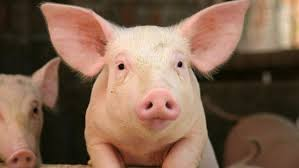
\includegraphics[scale=0.2]{images/pig.jpg}
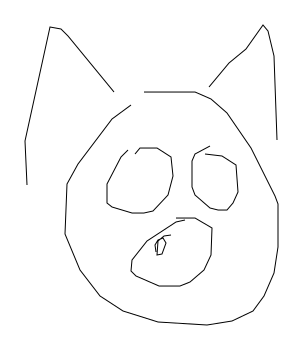
\includegraphics[scale=0.15]{images/pig00008.png}
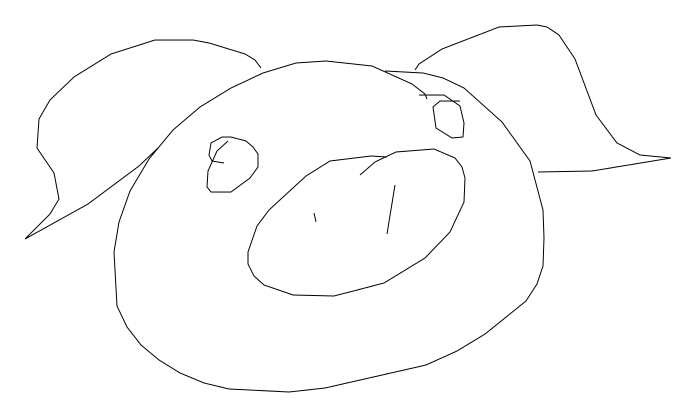
\includegraphics[scale=0.1]{images/pig00039.png}
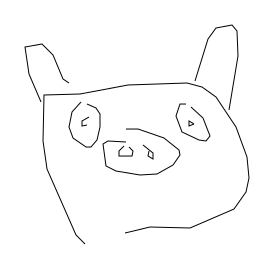
\includegraphics[scale=0.15]{images/pig00161.png}
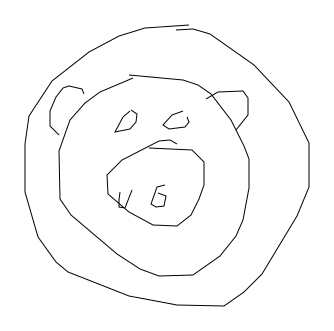
\includegraphics[scale=0.15]{images/pig00295.png}\\
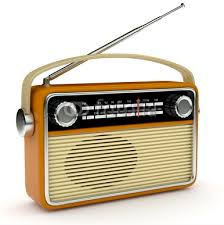
\includegraphics[scale=0.2]{images/radio.jpg}
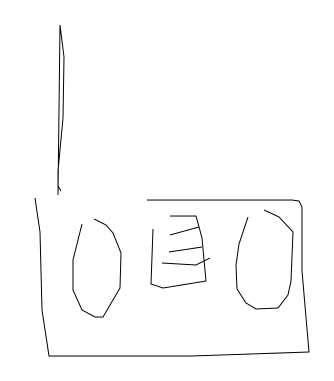
\includegraphics[scale=0.1]{images/radio00008.png}
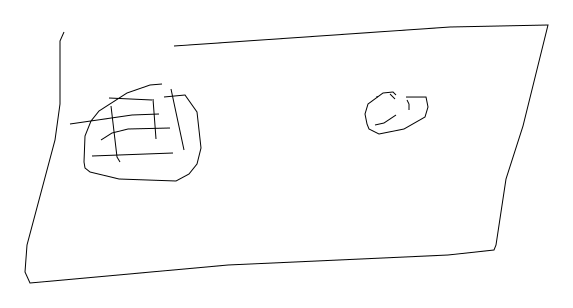
\includegraphics[scale=0.1]{images/radio00111.png}
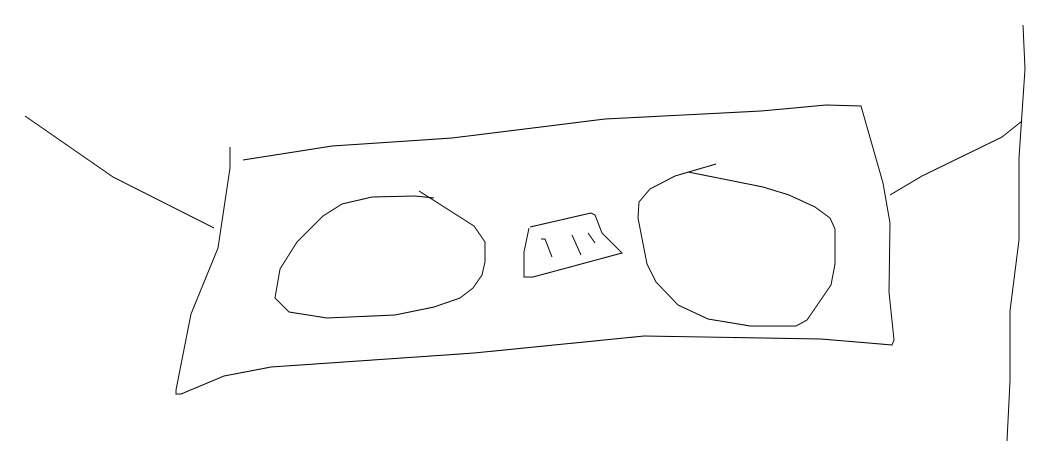
\includegraphics[scale=0.1]{images/radio00161.png}
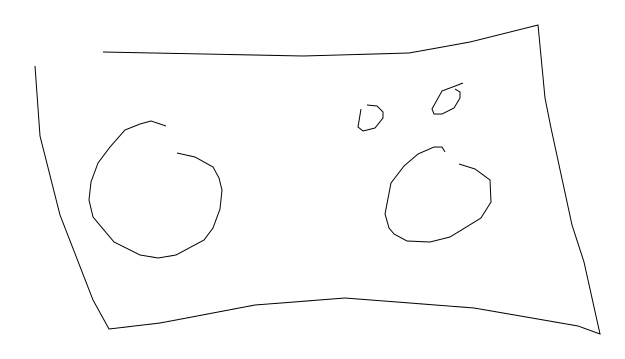
\includegraphics[scale=0.1]{images/radio00286.png}\\
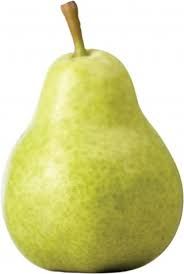
\includegraphics[scale=0.15]{images/pear.jpg}
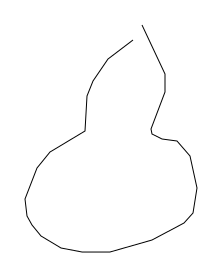
\includegraphics[scale=0.15]{images/pear00008.png}
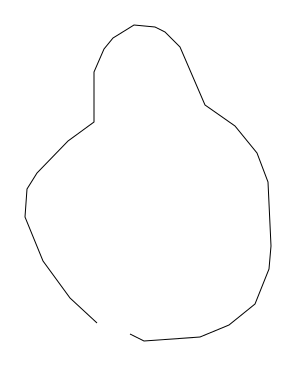
\includegraphics[scale=0.15]{images/pear00039.png}
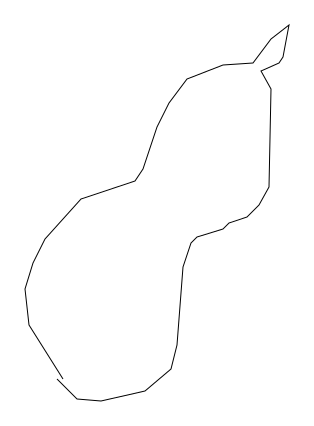
\includegraphics[scale=0.1]{images/pear00111.png}
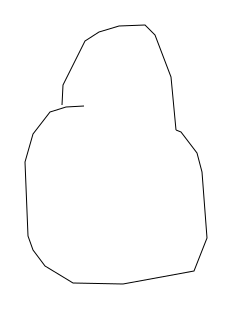
\includegraphics[scale=0.15]{images/pear00239.png}\\
\caption{Pixel images of a pear, pig, and radio collected from the web and their four sketches selected from the Quick Draw dataset \cite{quickdraw}}
\end{figure}


\section{Future works for final report}
The VAE restricts the latent variable z i.e. the output of the encoder to be from a unit Guassian distribution \cite{journals/corr/KingmaW13}. This allows for easier image generation because we know how to sample from a unit Guassian and that can be used to generate the sketches, unlike currently where we do not know the distribution of the latent variable. The adjustments needed for this change is to output the mean $\hat{\mu}$ and standard deviation $\hat{\sigma}$ from the CNN encoder instead of the latent variable and sample x from a unit Guassian i.e. $x\sim N(0, 1)$ so the hidden latent variable is $\hat{\mu} + x \hat{\sigma}$. To enforce that $\hat{\mu} + x \hat{\sigma}$ follow the unit Guassian, we can apply the Kullback–Leibler divergence loss on the mean $\hat{\mu}$ and standard deviation $\hat{\sigma}$ such that $L_{KL}(\hat{\mu}, \hat{\sigma}) = \frac{1}{2 N_{z}} (1 + \hat{\sigma} - \hat{\mu} - exp(\hat{\sigma}))$\cite{qdpaper} where $N_{z}$ is the number of dimensions of the latent vector $z$. Hence the overall loss becomes $L_{total}(s, \hat{s}) = L_{R}(s, \hat{s}) + L_{CE}(s, \hat{s}) + L_{KL}(\hat{\mu}, \hat{\sigma})$.

Another additional change could be to learn the distribution of the offsets $(\Delta x, \Delta y)$. The offsets $(\Delta x, \Delta y)$ could be modelled as a Gaussian mixture model (GMM) with M normal distributions\cite{DBLP:journals/corr/Graves13}. Hence instead of $(\Delta x, \Delta y)$ as the output from the LSTM, the output could be $(\pi, \mu_{x}, \mu_{y}, \sigma_{x}, \sigma_{y}, \rho_{xy})$ at each time step where $p(\Delta x, \Delta y) = \sum_{i=1}^{M} \pi_{i} \mathcal{N}(\Delta x_{i}, \Delta y_{i} | \mu_{x, i}, \mu_{y, i}, \sigma_{x, i}, \sigma_{y, i}, \rho_{xy, i})$ \cite{DBLP:journals/corr/Graves13}. With this change, the reconstruction loss $L_{R}$ would change to $L_{R} = \frac{1}{N-1} \sum_{t=0}^{N-1} log(p_{t}(\Delta x, \Delta y))$. Hence the offset could be sampled from the GMM instead directly calculated. This would allow a higher generalization of the pen strokes because the network learns the offset's distribution so we can sample the offset from the distribution instead. Since we sample from the offset's distribution, this allows more variation in the pen strokes hence there is more variation in the output sketches for improved learning.

Lastly, the third change could be the image features that we use. Instead of features from the final layer of the CNN, it would be wiser to use lower layers from CNN because the lower layers extract lower level features like edges which we want to be drawn by the sketches. Hence we could use the first couple of layers from the pre-trained network like VGG \cite{DBLP:journals/corr/SimonyanZ14a} where we could train the LSTM by holding the CNN with the VGG weights in the first phase then fine-tune the weights of the CNN in the second phase.


{\small
\bibliographystyle{abbrvnat}
\bibliography{egbib}
}

\end{document}